
\documentclass{beamer}
\usetheme{boxes}

\usepackage{tikz}

\begin{document}

\begin{frame}{}
\begin{center}
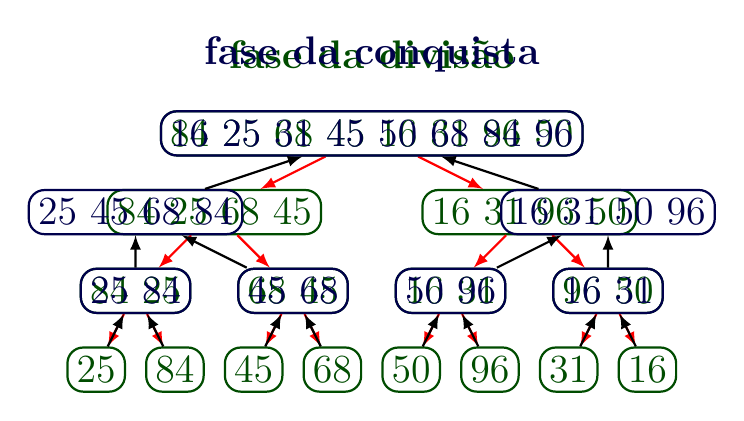
\begin{tikzpicture}
\def\D{2cm}
\def\dd{0}
\colorlet{divide color}{green!30!black}
\colorlet{conquer color}{blue!30!black}
\tikzset{
  scale=.8,
  every node/.style={font=\Large},
  divide path/.style={->,>=latex,red,thick,draw},
  divide/.style={divide color,rounded corners=2mm,thick,draw},
  conquer/.style={conquer color,rounded corners=2mm,thick,draw},
  conquer path/.style={->,>=latex,thick,draw},
}

%N
\node<1-4>[divide] (N) {84 25 68 45 16 31 96 50};
\node<1-4>[divide color] [above of=N] {\Large\bf fase da divis\~ao};
\node<5->[conquer color] [above of=N] {\Large\bf fase da conquista};
%N/2
 \def\dd{\D}
 \node<2-4>[divide] (N0) [below of=N, xshift=-\dd] {84 25 68 45};
 \node<2-4>[divide] (N1) [below of=N, xshift=\dd] {16 31 96 50};
%N/4
\def\dd{\D/2}
 \node<3-4>[divide] (N00) [below of=N0, xshift=-\dd] {84 25};
 \node<3-4>[divide] (N01) [below of=N0, xshift=\dd] {68 45};
 \node<3-4>[divide] (N11) [below of=N1, xshift=\dd] {96 50};
 \node<3-4>[divide] (N10) [below of=N1, xshift=-\dd] {16 31}; 
%N/8
\def\dd{\D/4}
\node<4->[divide] (N000) [below of=N00, xshift=\dd] {84};
\node<4->[divide] (N001) [below of=N00, xshift=-\dd] {25};
\node<4->[divide] (N010) [below of=N01, xshift=\dd] {68};
\node<4->[divide] (N011) [below of=N01, xshift=-\dd] {45};
\node<4->[divide] (N100) [below of=N10, xshift=\dd] {96};
\node<4->[divide] (N101) [below of=N10, xshift=-\dd] {50};
\node<4->[divide] (N110) [below of=N11, xshift=\dd] {16}; 
\node<4->[divide] (N111) [below of=N11, xshift=-\dd] {31}; 

%paths
\foreach \i in {0,1} {
  \path<2-4>[divide path] (N) -- (N\i);
}

\foreach \i in {0,1} {
 \foreach \j in {0,1} {
  \path<3-4>[divide path] (N\i) -- (N\i\j);
  }
}

\foreach \i in {0,1} {
 \foreach \j in {0,1} {
  \foreach \k in {0,1} {
  \path<4>[divide path] (N\i\j) -- (N\i\j\k);
  }
 }
}

% conquer
%N/4
\def\dd{\D/2}
 \node<5->[conquer] (C00) [below of=N0, xshift=-\dd] {25 84};
 \node<5->[conquer] (C01) [below of=N0, xshift=\dd] {45 68};
 \node<5->[conquer] (C10) [below of=N1, xshift=-\dd] {50 96};
 \node<5->[conquer] (C11) [below of=N1, xshift=\dd] {16 31}; 

\foreach \i in {0,1} {
 \foreach \j in {0,1} {
  \foreach \k in {0,1} {
  \path<5->[conquer path] (N\i\j\k) -- (C\i\j);
  }
 }
}

%N/2
\def\dd{\D}
 \node<6->[conquer] (C0) [above of=C01, xshift=-\dd] {25 45 68 84};
 \node<6->[conquer] (C1) [above of=C10, xshift=\dd] {16 31 50 96};

\foreach \i in {0,1} {
 \foreach \j in {0,1} {
  \path<6->[conquer path] (C\i\j) -- (C\i);
  }
}

%N
\def\dd{1.5*\D}
 \node<7>[conquer] (C) [above of=C0, xshift=\dd] {16 25 31 45 50 68 84 96};
\foreach \i in {0,1} {
  \path<7>[conquer path] (C\i) -- (C);
  }



\end{tikzpicture}

\end{center}
\end{frame}


\end{document}

